\section{Einleitung}
	\label{sec:einleitung}
	Dieser Versuch behandelt ged"ampfte und erzwungende Schwingungen am Beispiel des LC-Kreises.
	Schaltet man eine Induktivit"at mit einer Kapazit"at in Reihe, k"onnen sie ihre Energie periodisch austauschen (Abb \ref{fig:lc-kreis}).
	Durch einen Ohmschen Widerstand im Schaltkreis geht bei jedem Zyklus energie in Form von W"arme verloren und die Schwingung wird ged"ampft.
	Schlie"slich l"asst sich eine Schwingung anregen, indem man eine "au"sere, periodische Spannung anlegt.
	Hierbei treten verschiedene Resonanzph"anomene auf.
	
	\begin{figure}[h!]
		\centering
		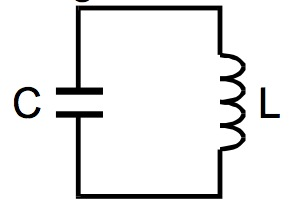
\includegraphics[width = 5cm]{img/lc-kreis.JPG}
		\caption{Ein LC-Kreis: Energie, die im System vorhanden ist, wird periodisch zwischen Kondensator und Spule ausgetauscht. \cite{anleitung}}
		\label{fig:lc-kreis}
	\end{figure}

\section{Theorie}
	\label{sec:theorie}

	Der hier behandelte Aufbau l"asst sich mit den Kirchhoff'schen Regeln durch Differentialgleichungen 2. Ordung beschreiben.
	Die Struktur dieser Gleichung ist bei jeder ged"ampften Schwingung gleich, weshalb die Ergebnisse leicht auf andere Probleme "ubertragen werden k"onnen (z.B. Sto"sd"ampfer).

	\subsection{Ged"ampfte harmonische Schwingung}

	F"ur den LC-Schwingkreis l"asst sich folgende Gleichung aufstellen:

	\begin{equation*}
		\frac{\partial^2}{\partial t^2} I + \frac{R}{L} \frac{\partial}{\partial t} I + \frac{1}{LC} I = 0
	\end{equation*}

	Es bezeichnen $R$ den Widerstand des Kreises, $L$ die Induktivit"at der Spule und $C$ die Kapazit"at des Kondensators.

	Der Ansatz 

	\begin{eqnarray*}
		I(t) & = & Ae^{\omega t} \nonumber \\
		\Rightarrow \quad \omega & = & - \frac{R}{2L} \pm \sqrt{\frac{R^2}{4L^2} - \frac{1}{LC}}
	\end{eqnarray*}

	liefert drei verschiedene Arten der Schwinung. Au"serdem erkennt man, dass diese Gleichung f"ur den unged"ampften Fall -- also $R = 0$ -- eine harmonische Schwingung mit der Frequenz $1/\sqrt{LC}$ ergibt.
	Die Amplitude $A$ bezeichnet im Folgenden eine Konstante, die von den Anfangsbedingungen abh"angt.

	\subsubsection{Schwingfall $\frac{R^2}{4L^2} < \frac{1}{LC}$}
		Beim Schwingfall dominiert die Harmonische Schwingung.
		Die Amplitude der Schwingung nimmt jedoch allm"ahlich ab.
		Abbildung \ref{amplitude} zeigt den Verlauf der Schwingung.
		Die L"osung lautet dann

		\begin{equation*}
			I(t) = A e^{-\frac{R}{2L}} e^{\pm i \sqrt{\frac{1}{LC}- \frac{R^2}{4L^2}}}.
		\end{equation*}

	\subsubsection{Aperiodischer Grenfall $\frac{R^2}{4L^2} = \frac{1}{LC}$}
		In diesem Fall kehrt die Amplitude schnellstm"oglich zur Ausgangslage zur"uck.
		Es tritt keine Schwingung auf.
		Dieser Fall ist in Abbildung \ref{fig:aperiodischer_fall} als gestrichelte Linie eingezeichnet.
		Die L"osung lautete hier

		\begin{equation*}
			I(t) = A e^{-\frac{R}{2L}}.
		\end{equation*}

	\subsubsection{"Uberd"ampfung oder Kriechfall $\frac{R^2}{4L^2} > \frac{1}{LC}$}
		In diesem Fall n"ahert sich die Amplitude besonders langsam der Ruhelage.
		Diese wird erst nach einem Nulldurchgang oder einem vorl"aufigen Ausschlag erreicht.
		Die L"osung lautet

		\begin{equation*}
			I(t) = Ae^{-\frac{R}{2L} \pm \sqrt{\frac{R^2}{4L^2} - \frac{1}{LC}}}
		\end{equation*}

		und wird exemplarisch durch die farbigen Graphen in Abbildung \ref{fig:aperiodischer_fall} visualisiert.

		\begin{figure}[h!]
			\centering
			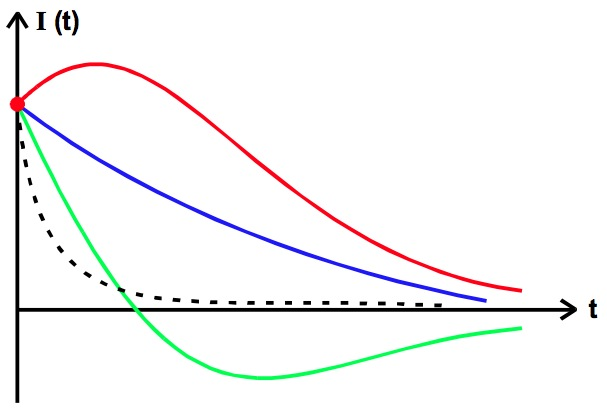
\includegraphics[width = 10cm]{img/aperiodisch.JPG}
			\caption{Verl"aufe des Aperiodischen Grenzfalles (gestrichelt) und des Kriechfalles. \cite{anleitung}}
			\label{fig:aperiodischer_fall}
		\end{figure}

	\subsection{Erzwungene Schwingungen}

		Durch eine "au"sere periodische Spannung $U(t) = U_0 e^{i\omega t}$ l"asst sich eine Schwingung im Kreis erzwingen.
		Die Kirchhoff'schen Regeln liefertn hier die Differentialgleichung f"ur die Kondensatorspannung $U_\mathrm{C}$

		\begin{equation*}
			\frac{\partial^2}{\partial t^2} U_\mathrm{C} + \frac{R}{L} \frac{\partial}{\partial t} U_\mathrm{C} + \frac{1}{LC} U_\mathrm{C} = U_0 e^{i \omega t}.
		\end{equation*}

		Zur L"osung dieser Gleichung wird der homogene und der partikul"are Teil gel"ost.
		Nach gen"ugend gro"ser Zeit ist der homogene Teil, welcher den Einschwingvorgang beschreibt, zu vernachl"assigen, weshalb die Schwingung durch den Partikul"arteil

		\begin{equation*}
			U_\mathrm{C} (\omega, t) = U(\omega)e^{i \omega t + \varphi}
		\end{equation*}

		beschrieben werden kann.
		Hier gelten die Zusammenh"ange

		\begin{eqnarray*}
			U(\omega) & = & \frac{U_0}{\sqrt{\left( 1 - LC \omega^2 \right)^2 + \left( \omega RC\right)^2}}, \\
			\tan{\varphi} & = & \frac{-\omega RC}{1 - LC\omega^2}.
		\end{eqnarray*}

		Der Wert $\varphi$ gibt hiertbei den Phasenunterschied zwischen Erregerspannung $U(t)$ und Resonator, also der Kondensatorspannung $U_\mathrm{C}$ an.

		Bemerkenswert ist, dass die Spannung $U(\omega)$ bei einer bestimmten Frequenz -- der Resonanzfrequenz $\omega_\mathrm{res}$ -- einen maximalen Wert annimmt.
		Es gilt

		\begin{equation*}
			\omega_\mathrm{res} = \sqrt{\frac{1}{LC}-\frac{R^2}{2L^2}}.
		\end{equation*}

		F"ur den besonderen Fall der schwachen D"ampfung gilt

		\begin{eqnarray*}
			\frac{R^2}{2L^2} & \ll & \frac{1}{LC} \\
			\Rightarrow \quad U_\mathrm{C} \quad = \quad \frac{1}{\omega_0 RC} & = & \frac{1}{R} \sqrt{\frac{L}{C}} U_0 \quad = \quad q U_0.
		\end{eqnarray*}

		Mit der Eigenfrequenz $\omega_0 = 1/\sqrt{LC}$.
		Wenn der Widerstand $R$ also gegen Null geht, kann $U_\mathrm{C}$ unendlich verst"arkt werden.
		Diesen Fall nennt man Resonanzkatastrophe.

		Der Vorfaktor $q$ wird als G"ute des Schwingkreises bezeichnet.
		Mit den Frequenzen $\omega_+$ und $\omega_-$, die die Frequenzen bezeichnen bei denen $U(\omega)$ gerade den Bruchteil $1/\sqrt{2}$ annimmt, gilt zudem

		\begin{equation*}
			q = \frac{\omega_0}{\omega_+ - \omega_-}.
		\end{equation*}

		Im Gegensatz dazu steht die starke D"ampfung:

		\begin{equation*}
			\frac{R^2}{2L^2} \gg \frac{1}{LC}.
		\end{equation*}

		Nun geht $U_\mathrm{C}$ f"ur wachsende Frequenzen monoton gegen Null.

	\subsection{Scheinwiderstand}
		Induktivit"aten und Kapazit"aten besitzen komplexe Widerst"ande.
		Sie haben die Besonderheit, dass sie von der Frequenz des Stromkreises und vom Winkel zwischen Real- und Imagin"arteil des Widerstandes abh"angt.
		Beide Zusammenh"ange lassen sich visualisieren und sind in Abbildungen \ref{z_frequenz} und \ref{z_winkel} jeweils f"ur die Betr"age der Widerst"ande dargestellt.

		\begin{figure}[h]
			\centering
			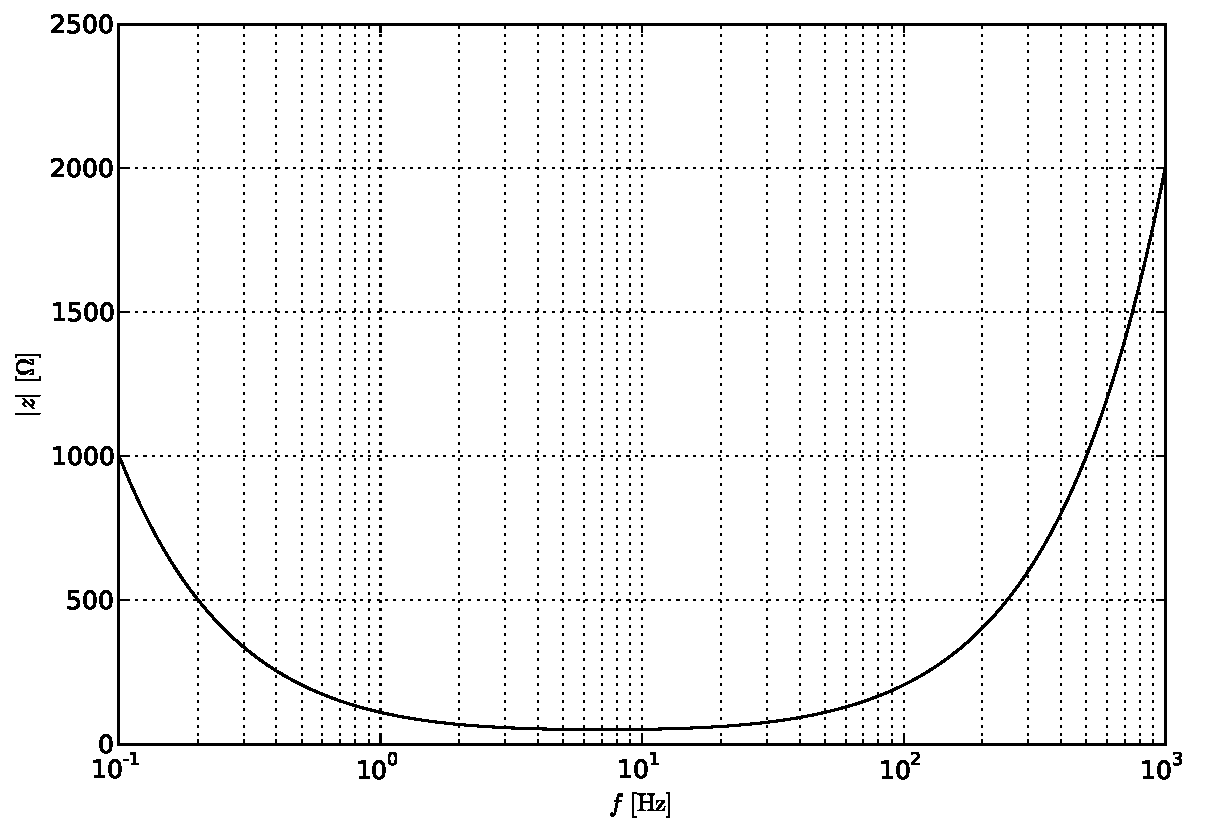
\includegraphics[width = 10cm]{img/z_f.pdf}
			\caption{Theoretischer Verlauf von $|z|$ im Serienschwingkreis bei $R = \SI{50}{\ohm}$, $C = \SI{10}{\milli \farad}$ und $L = \SI{2}{\henry}$.}
			\label{z_frequenz}
		\end{figure}

		\begin{figure}[h]
			\centering
			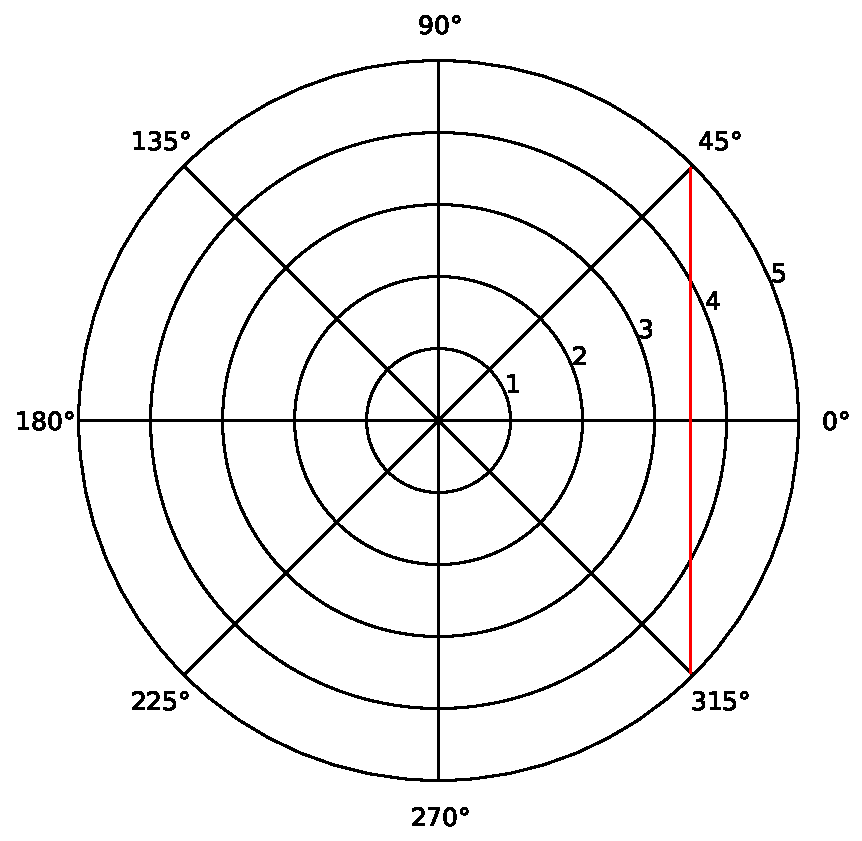
\includegraphics[width = 10cm]{img/z_phi.pdf}
			\caption{Theoretischer Verlauf von $|z|$ (rot) im Serienschwingkreis bei $R = \SI{3.5}{\ohm}$.}
			\label{z_winkel}
		\end{figure}
		\clearpage